\documentclass[12pt]{article}

\usepackage{booktabs}
\usepackage{tabularx}
\usepackage{hyperref}
\usepackage{graphicx}
\usepackage[a4paper, margin=0.75in]{geometry}
\usepackage{subcaption}
\usepackage{float}
\usepackage{amssymb}
\usepackage[table]{xcolor}
\usepackage{enumitem}
\usepackage{pgfplots}
\pgfplotsset{compat=1.18}
\usepackage{tikz}


\hypersetup{
    colorlinks=true,       % false: boxed links; true: colored links
    linkcolor=red,          % color of internal links (change box color with linkbordercolor)
    citecolor=green,        % color of links to bibliography
    filecolor=magenta,      % color of file links
    urlcolor=cyan           % color of external links
}

\title{Norman's Principles Report\\\progname}

\author{\authname}

\date{}

\input{../../Comments}
\input{../../Common}

\begin{document}

\maketitle
\thispagestyle{empty}

~\newpage

\pagenumbering{arabic}

\begin{table}[hp]
\caption{Revision History} \label{TblRevisionHistory}
\begin{tabularx}{\textwidth}{llX}
\toprule
\textbf{Date} & \textbf{Developer(s)} & \textbf{Change}\\
\midrule
04-06-2026 & Virochaan Ravichandran Gowri & Norman's Principles Final Version\\

... & ... & ...\\
\bottomrule
\end{tabularx}
\end{table}

~\newpage

\tableofcontents

~\newpage

\pagenumbering{arabic}
\section{Introduction}
This report evaluates the final MES Event Management System using Norman's Design Principles as a usability benchmark. The goal is to identify where the current design supports intuitive interaction and where it creates friction for users. For each principle, we analyze concrete examples from both the user portal and the admin portal, explain why each example is considered a strong or weak application of the principle, and provide recommendations for improvement where needed.

The discussion is grounded in observations from usability testing and day-to-day platform workflows as well as general overview of the application as a whole. Screenshots are referenced alongside each example to show the specific interface elements being evaluated.

\section{Visibility}
Visibility concerns whether users can immediately understand what actions are available and where to perform them just by looking at the interface.

\subsection{Example 1 (Good): Clear top-level User Portal navigation}
In the user portal, the top-level navigation structure makes major areas of the platform immediately visible. This supports fast orientation, especially for first-time users, because users can scan the page and quickly identify the section they need. We consider this a good application of visibility because available actions are not hidden behind extra clicks or ambiguous labels. The Navbar also has highlighted states to show what tab you currently on so the user has better clarity. 

\begin{figure}[H]
    \centering
    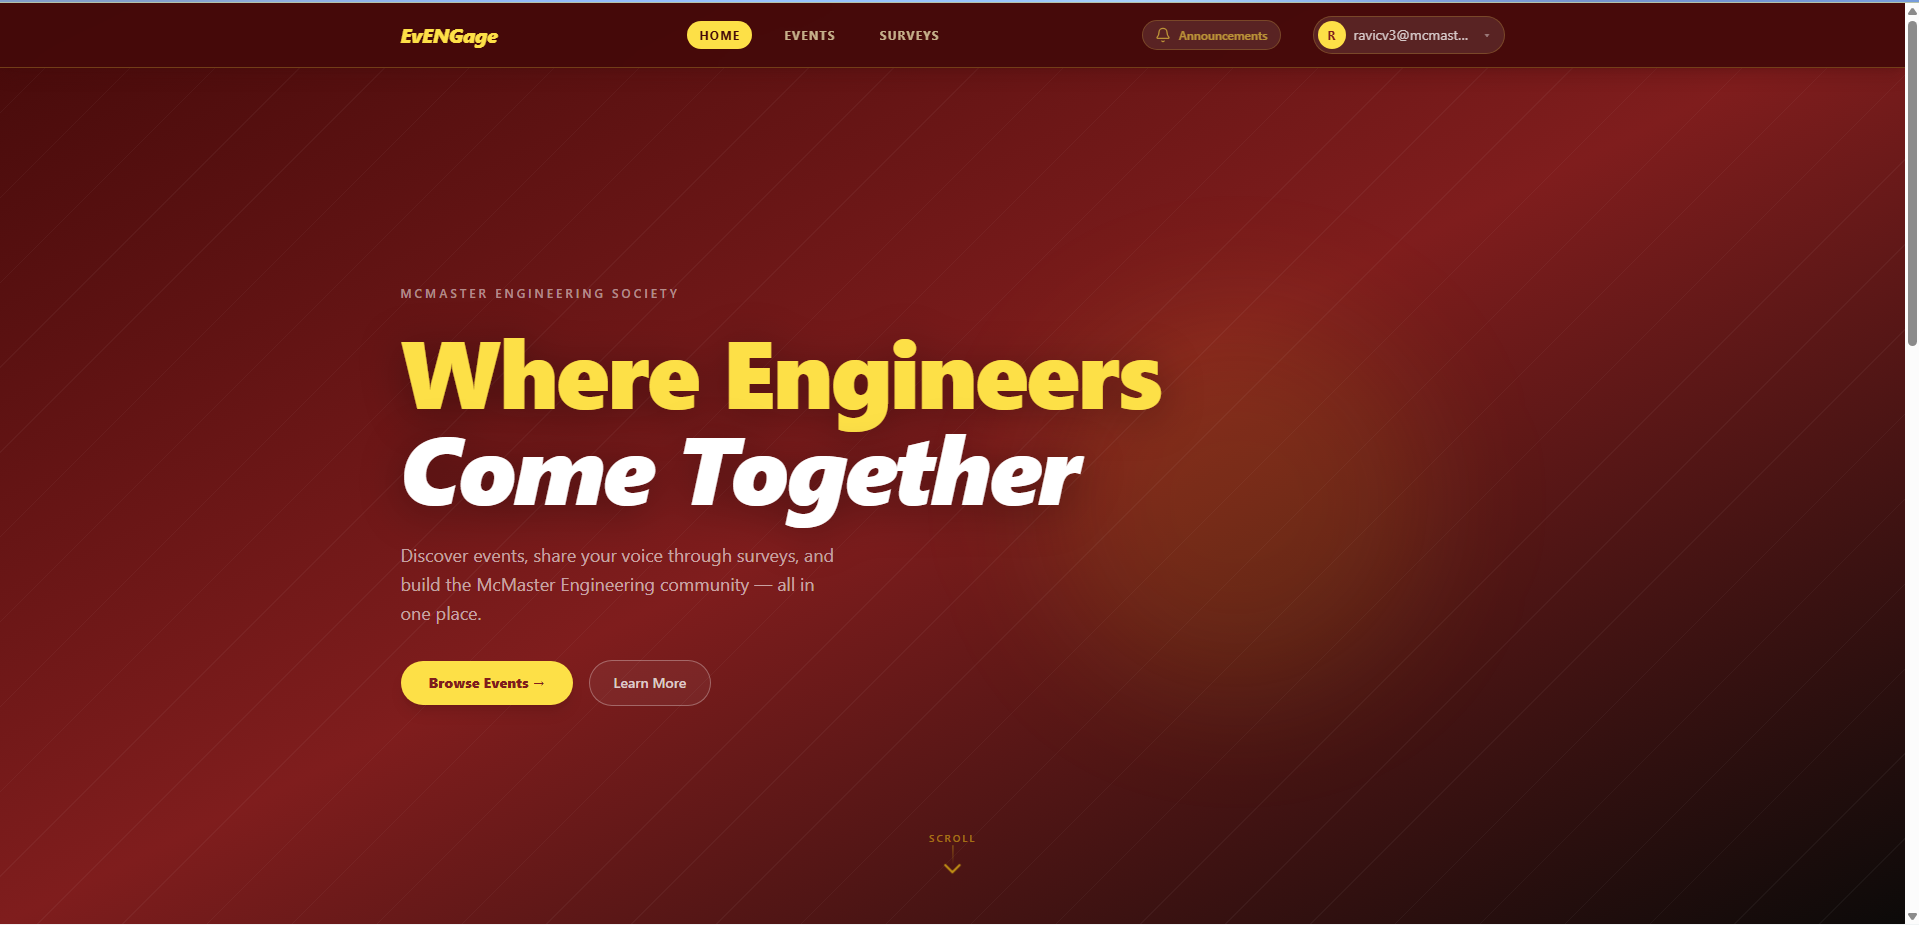
\includegraphics[width=0.9\textwidth]{Images/Visibility1.png}
    \caption{User Portal Home Page with Top Navbar}
    \label{fig:user-portal-home-tab}
\end{figure}

\subsection{Example 2 (Good): Banner forcing Profile Setup}
In the user portal, new accounts are shown a large, high-contrast banner that clearly prompts profile setup before users continue with normal platform use. This is a good application of visibility because the next required action is placed prominently at the top of the workflow, making it difficult to miss. Testers were able to quickly understand what step was pending and where to click, which reduced confusion during first-time onboarding. Other actions are also locked behind this setup of the profile further emphasizing its importance.
\begin{figure}[H]
    \centering
    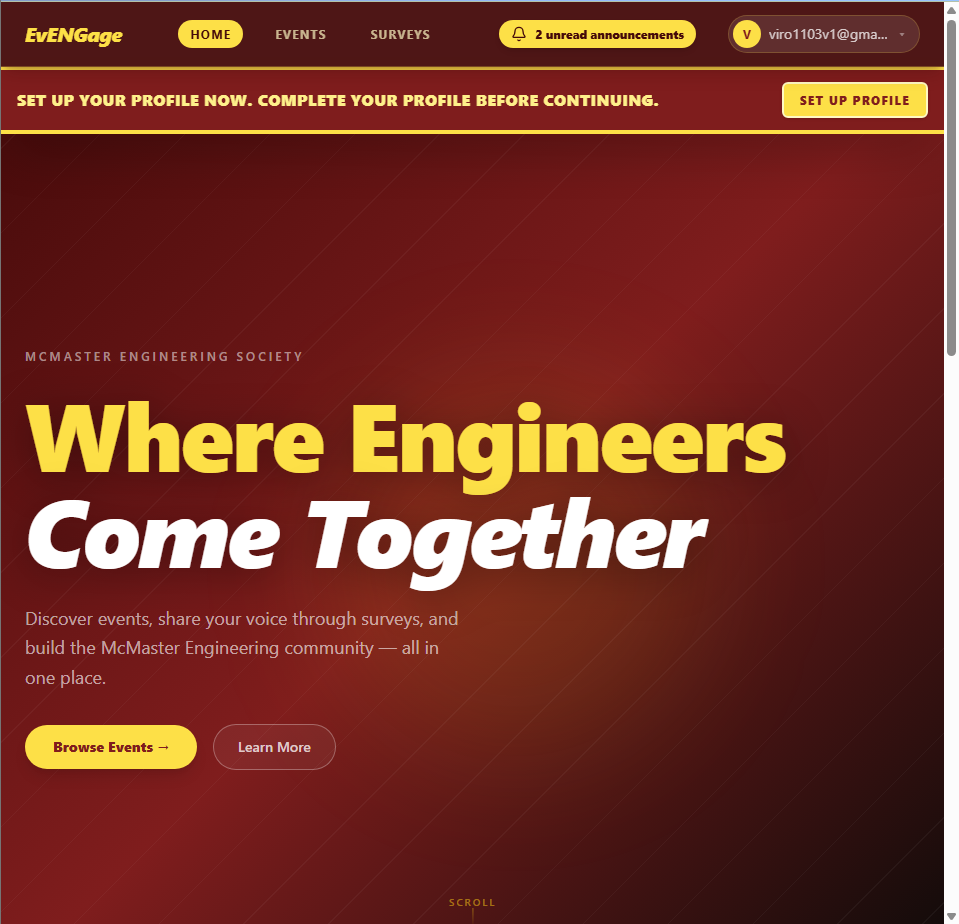
\includegraphics[width=0.9\textwidth]{Images/Visibility2.png}
    \caption{User Portal Home Page with Top Navbar}
    \label{fig:user-portal-home-tab}
\end{figure}
\subsection{Example 3 (Bad): Notification not fully visible}
Announcements are currently shown in a relatively small section of the user interface, which makes important updates easy to overlook during normal browsing. Testers often focused on event cards and primary actions, and some missed the notifications unless they were explicitly told where to look. This is a poor application of visibility because critical information is present but not prominent enough to reliably attract attention.
\begin{figure}[H]
    \centering
    
\includegraphics[width=0.9\textwidth]{Images/Visibility3.png}
    \caption{User Portal Home Page with Top Navbar}
    \label{fig:user-portal-home-tab}
\end{figure}
\textbf{Recommendation:} Increase announcement visibility by promoting urgent notices to a larger, high-priority banner area, adding unread indicators, and using stronger visual hierarchy so users can immediately identify new or important updates. We could also make the announcements itself into a seperate tab or make it much more present so that user's cannot avoid it. Also it would make it easier for them to reaccess the announcements if neccesary.


\section{Feedback}
Feedback concerns whether the system clearly communicates the result of a user's action.

\subsection{Example 1 (Bad): Registering for unpaid events lacks a dedicated confirmation screen}
In the current user portal flow, unpaid registrations end with a small success toast and an updated button state, but users are not taken to a dedicated confirmation page that summarizes what happened. This is a weak application of Norman's Feedback principle because after a high-importance action users should receive clear confirmation that the system accepted their request. During usability testing, several users moved back to the events list to verify whether registration was successful, which indicates that the feedback is present but not strong enough to fully close the interaction.
\begin{figure}[H]
    \centering
    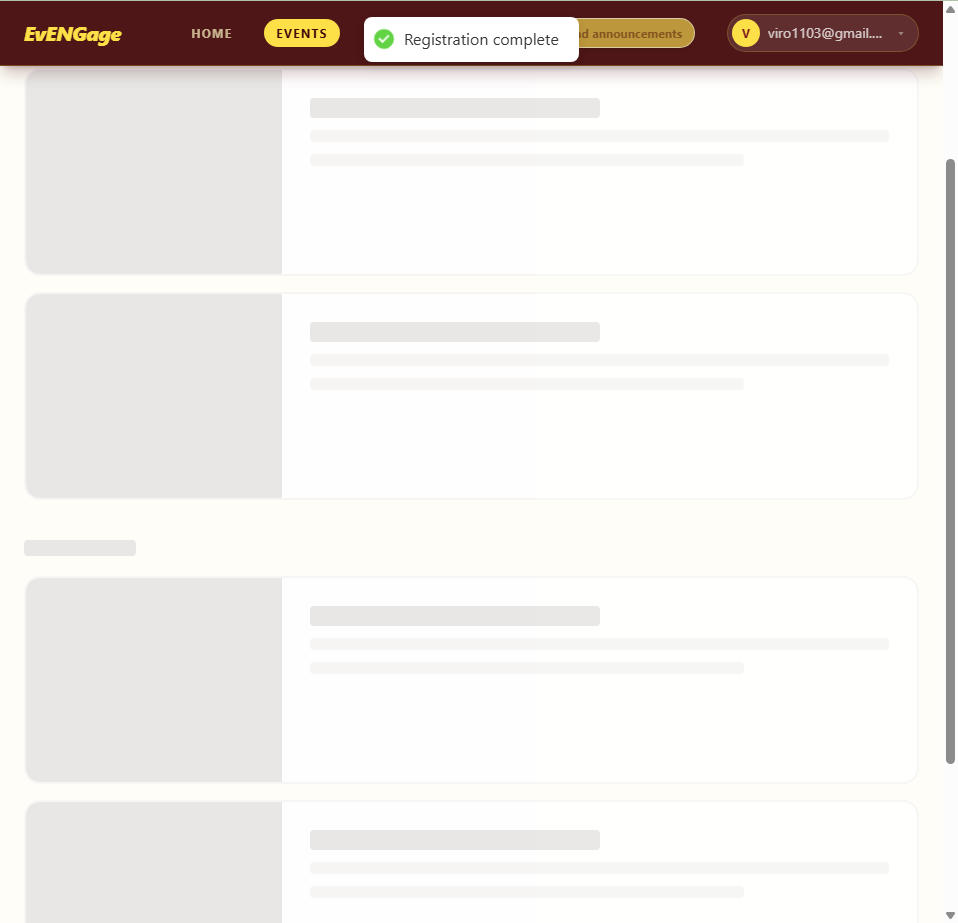
\includegraphics[width=0.9\textwidth]{Images/Feedback1.png}
    \caption{User Portal unpaid event registration completion state}
    \label{fig:feedback-unpaid-registration}
\end{figure}
\textbf{Recommendation:} Add a dedicated post-registration confirmation page for unpaid events that is similar to the paid flow result screen that includes the event details and clear post success actions such as navigation to other pages. This would make the system response more explicit, reduce uncertainty, and improve user confidence that the action completed successfully.

\subsection{Example 2 (Good): Survey Submission Confirmation}
The platform applies Feedback well when users submit surveys in the user portal. After a response is submitted, users receive immediate confirmation that their survey response was recorded and the survey no longer appears under Available Surveys instead moving into Completed Surveys. This gives both instant feedback and persistent feedback in the navigation flow. Under the completed surveys you cannot resubmit and you can only use edit and delete submissions button ensuring the the user can still see that the form has been submitted.

This is a strong application of Norman's Feedback principle because users can clearly tell that the action completed successfully and can verify the result later without re-submitting. The transition from available to completed state also reduces uncertainty about whether the platform saved their responses. 

\begin{figure}[H]
    \centering
    \begin{subfigure}[t]{0.48\textwidth}
        \centering
        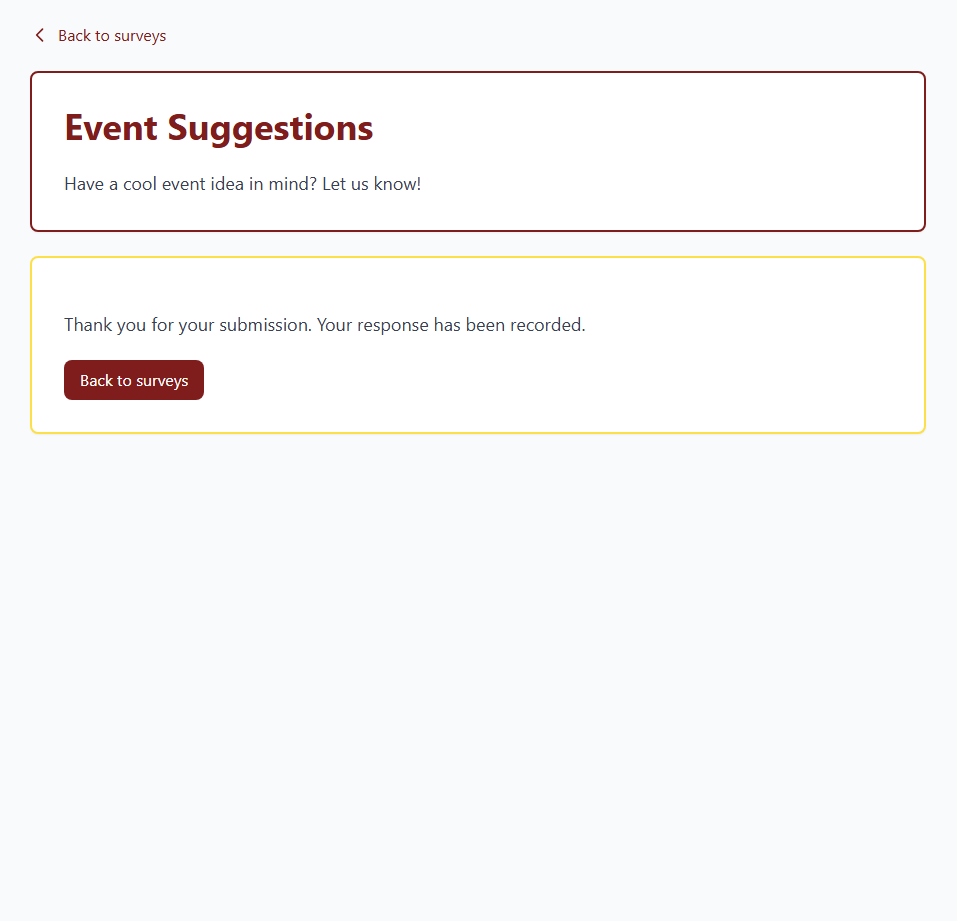
\includegraphics[width=\textwidth]{Images/Feedback2.1.png}
        \caption{Survey Submitted Page}
        \label{fig:feedback-survey-submission-left}
    \end{subfigure}
    \hfill
    \begin{subfigure}[t]{0.48\textwidth}
        \centering
        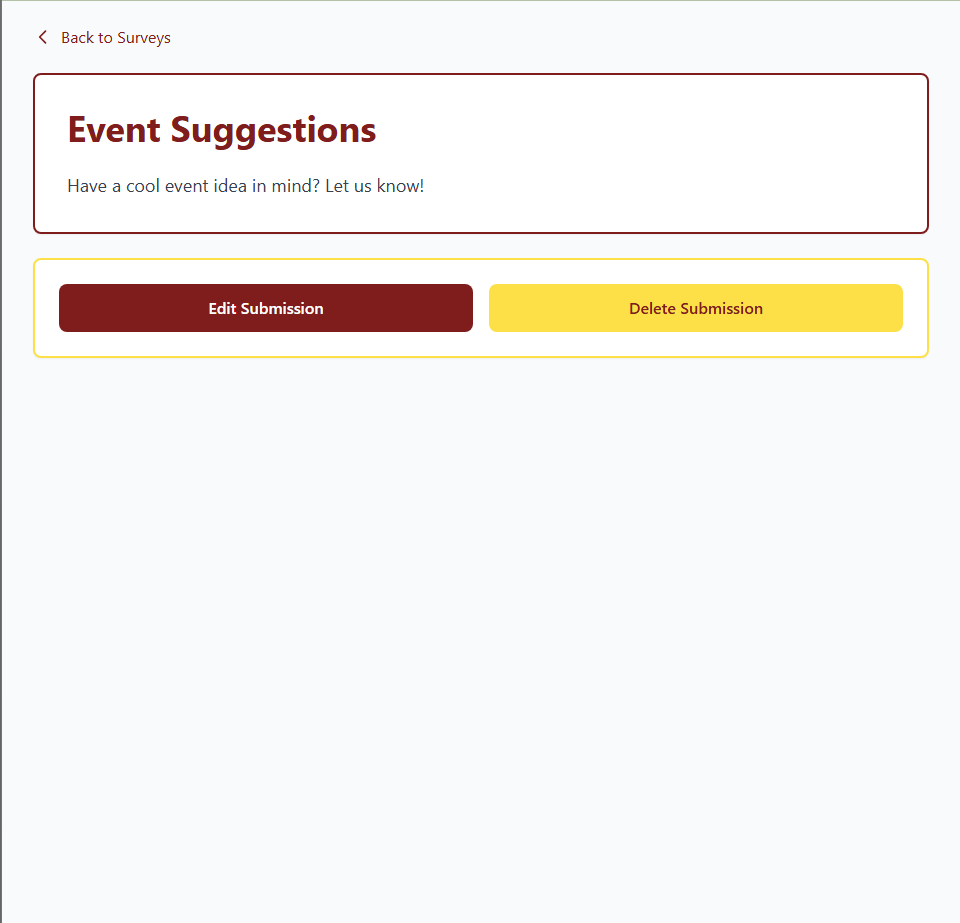
\includegraphics[width=\textwidth]{Images/Feedback2.png}
        \caption{Survey in Completed Surveys}
        \label{fig:feedback-survey-submission-right}
    \end{subfigure}
    \caption{User Portal survey submission feedback and completed state}
    \label{fig:feedback-survey-submission}
\end{figure}

\subsection{Example 3 (Bad): Admin Portal Event Creation}
In the admin portal's event creation flow, successful submission closes the modal and refreshes the list, but there is no explicit success confirmation message to verify that the event was created. This is a weak use of Feedback because after a high-impact administrative action, users should receive direct confirmation rather than having to infer success from a list update. \\
\\
\textbf{Recommendation:} After successful event creation, display a visible success message (for example, ``Event created successfully'') and provide an optional direct action such as View or Edit Event. This would make completion feedback explicit and reduce ambiguity for users on what the next steps they can proceed with are.


\section{Affordance}
Affordance concerns whether the appearance of an interface element suggests how it should be used.

\subsection{Example 1 (Good): Announcements bell clearly suggests notification access}
In the user portal header, the announcements control uses a bell icon with a high constrast notification status when new messages exist. This visual design strongly implies that a new announcements exists and entices the user into clicking there. It also matches common interface conventions users already recognize because this same pattern is used in various locations. This is a good application of affordance because the element looks interactive and communicates purpose before the user clicks it. The stronger styling for unread announcements also hints that the control deserves immediate attention.

\begin{figure}[H]
    \centering
    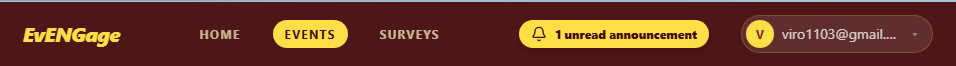
\includegraphics[width=0.9\textwidth]{Images/Affordance1.png}
    \caption{User portal announcements bell with unread emphasis}
    \label{fig:affordance-announcements-bell}
\end{figure}

\subsection{Example 2 (Good): Publish/Unpublish controls in form builder communicate state and action}
In the admin form builder, publish controls are presented as clear action buttons paired with visible status indicators (for example, published/unpublished and locked/unlocked states). This makes it easy for admins to infer both what the current state is and what action the button will perform next. This is a strong affordance pattern because the visual design links control appearance with system state. Users can predict the consequence of interaction without needing extra documentation.

\begin{figure}[H]
    \centering
    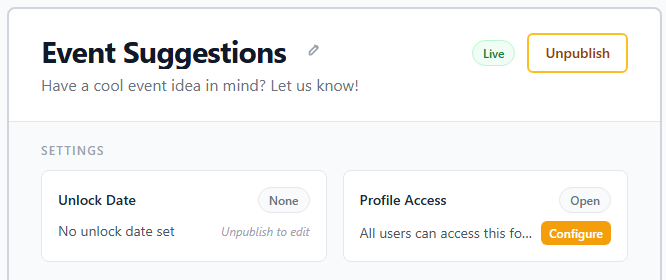
\includegraphics[width=0.9\textwidth]{Images/Affordance2.png}
    \caption{Admin form builder publish controls and state indicators}
    \label{fig:affordance-publish-controls}
\end{figure}

\subsection{Example 3 (Bad): Collapsed admin sidebar reduces navigation affordance}
When the admin sidebar is collapsed, most navigation labels disappear and only icons remain. While experienced users may still recognize the icons, new or infrequent users may struggle to infer each destination quickly. Though the icons used are the commonly  This is a weaker application of affordance because the controls remain clickable but their purpose becomes less obvious without text labels. The interface relies more on memory than on self-explanatory design.

\begin{figure}[H]
    \centering
    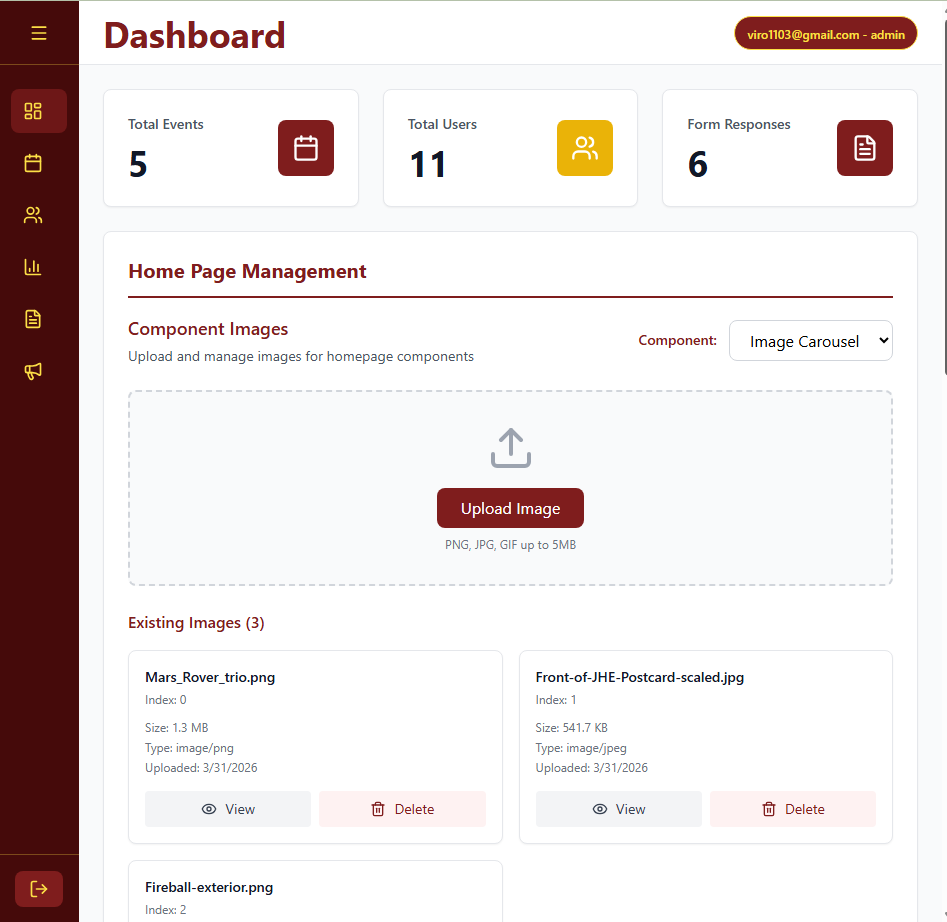
\includegraphics[width=0.9\textwidth]{Images/Affordance3.png}
    \caption{Admin sidebar in collapsed icon-only mode}
    \label{fig:affordance-collapsed-sidebar}
\end{figure}

\textbf{Recommendation:} Improve collapsed sidebar affordance by adding persistent icon tooltips, optional short labels on hover, or a partially collapsed mode that retains abbreviated text. All these method keep the text based nature so there is no ambiguity on where the different tabs lead to. We can also ensure the at the tabs open in the expanded state not the collapsed state as this solves the issues for first time users and limits the problems of them having to perform unneccesary actions.

\section{Mapping}
Mapping concerns whether the relationship between a control and its effect is natural and understandable.

\subsection{Example 1 (Good): Publish/Unpublish control maps directly to form availability}
In the admin form builder, the publish toggle and status pill create a direct and easy-to-understand mapping between control and system state. Selecting Publish makes the form live and constrained for editing, while selecting Unpublish returns the form to an editable state. The status indicators reinforce this relationship immediately. This is a strong application of Mapping because admins can accurately predict the outcome of each action before clicking.

\begin{figure}[H]
    \centering
    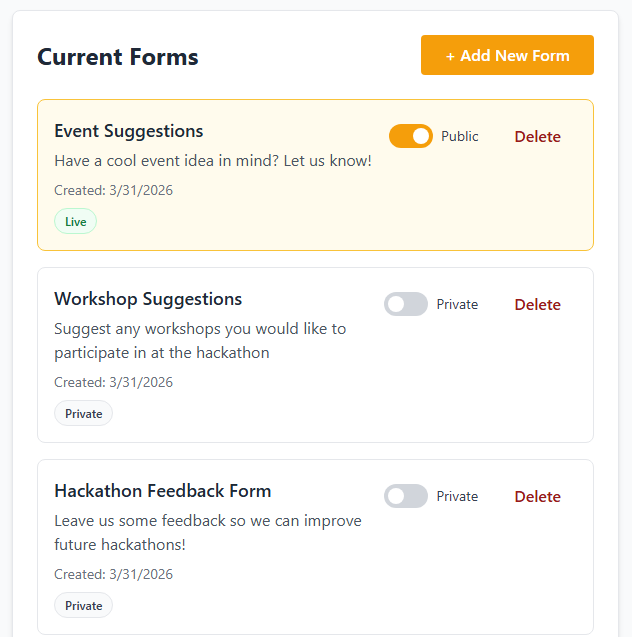
\includegraphics[width=0.9\textwidth]{Images/Mapping1.png}
    \caption{Admin form builder publish and status controls}
    \label{fig:mapping-publish-unpublish}
\end{figure}

\subsection{Example 2 (Bad): Event details page has weak control-to-result mapping for sharing}
On the event details page, the Share Event control appears beside the primary registration action, but the resulting behavior is not clearly communicated before interaction. Users can identify that the button is clickable, but it is unclear whether it will copy a link, open a modal, or trigger another sharing flow. This is a weak application of Mapping because the control does not clearly indicate its exact effect, forcing users to click first and interpret the result afterward.

\begin{figure}[H]
    \centering
    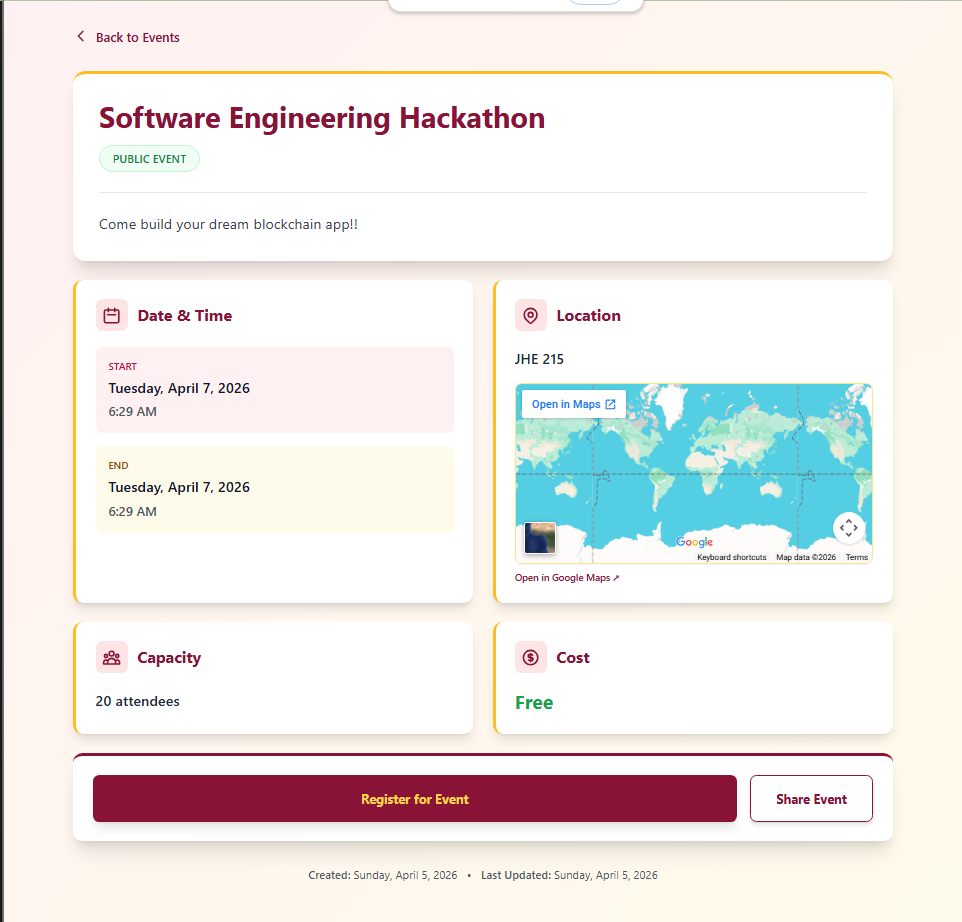
\includegraphics[width=0.9\textwidth]{Images/Mapping2.png}
    \caption{Event details controls where share action outcome is not explicitly mapped}
    \label{fig:mapping-share-control}
\end{figure}

\textbf{Recommendation:} Rename the control to a more explicit label such as Copy Event Link or Share via, and provide immediate post-click feedback. This would make the control-to-result mapping clearer and reduce ambiguity about what the action actually does.

\subsection{Example 3 (Bad): Opening announcements also marks them as read}
In the user portal, opening the announcements panel automatically marks unread items as read after a short delay. This creates a weaker mapping because the visible user action (open to view) also triggers a state-changing side effect (mark as read) that may not match user intent. This is a weak application of Mapping since one control interaction implicitly performs two different effects, making the outcome less predictable.

\begin{figure}[H]
    \centering
    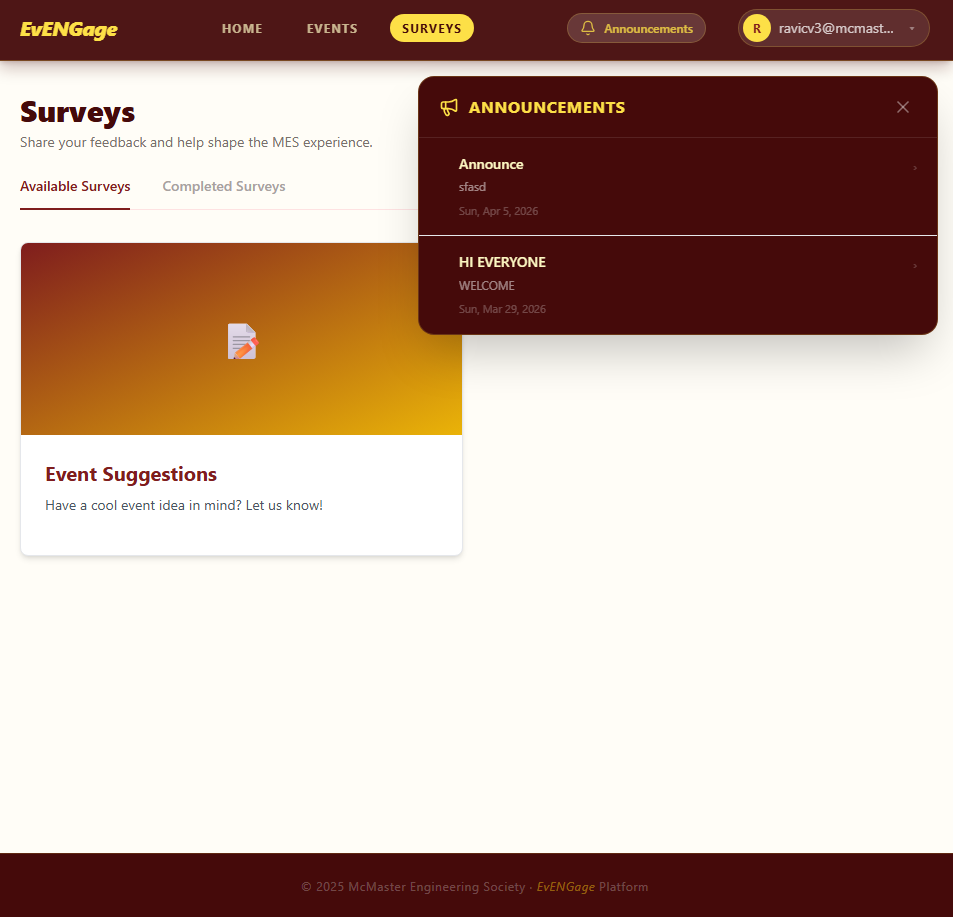
\includegraphics[width=0.9\textwidth]{Images/Mapping3.png}
    \caption{Announcements open action causing both view and read-state changes}
    \label{fig:mapping-announcements-read-state}
\end{figure}

\textbf{Recommendation:} Separate these effects by keeping open announcements as a view-only action and adding an explicit Mark all as read control or having the read action be linked to actually clicking on the announcement causing the read action to be done. This would make control-to-effect mapping more transparent and user-driven rather than having multiple actions integrated into one when that may not be the user intention.


\section{Constraints}
Constraints concern how the system limits incorrect actions and guides users toward valid ones.

\subsection{Example 1 (Good): Features locked on published forms}
In the admin form builder, once a form is published, editing controls for questions and profile access rules are constrained until the form is unpublished. The interface provides clear cues such as disabled controls and warnings like `Unpublish the form before modifying questions.' This is a strong application of Norman's Constraints principle because it prevents admins from making structural changes that could invalidate active submissions or create inconsistent form behavior for users.

This constraint also guides the correct workflow: configure first, publish when stable, and unpublish before making major edits. By enforcing this sequence the platform reduces accidental misconfiguration and protects data integrity across ongoing survey responses.

\begin{figure}[H]
    \centering
    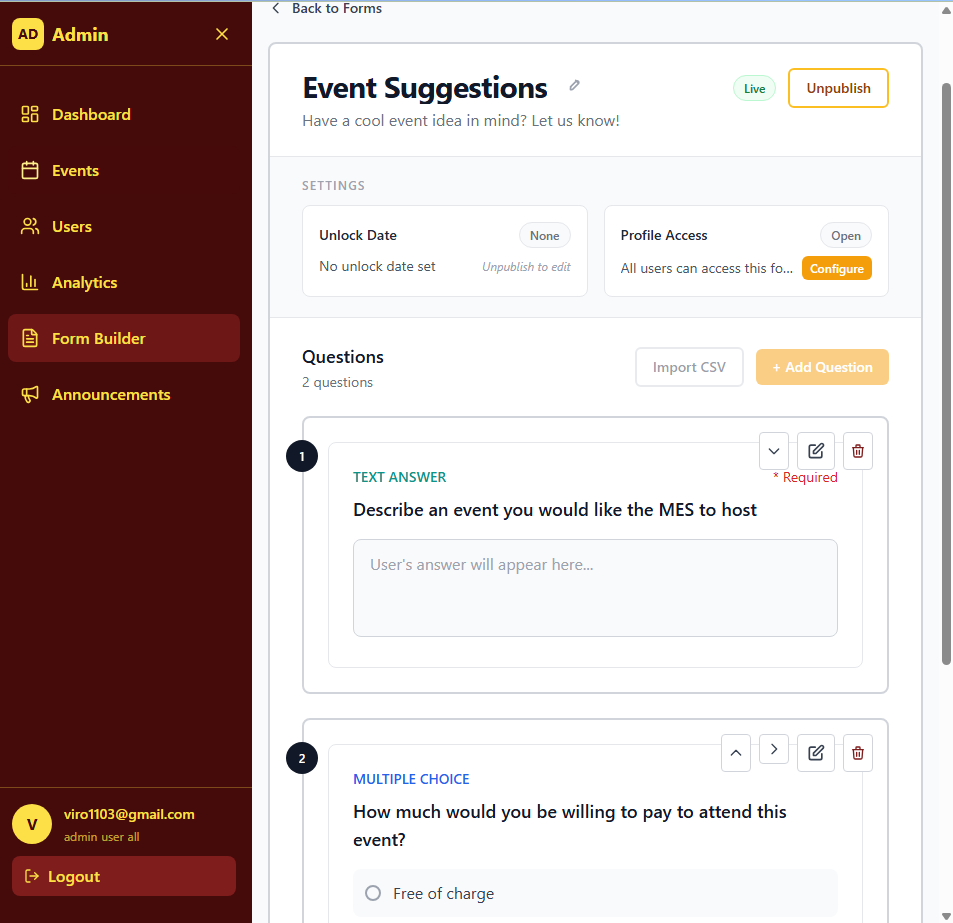
\includegraphics[width=0.9\textwidth]{Images/Constraints1.png}
    \caption{Admin form builder constraints requiring unpublish before editing}
    \label{fig:constraints-published-form-lock}
\end{figure}

\subsection{Example 2 (Good): Event and survey participation is constrained until profile completion}
In the user portal, the system prevents users from registering for events or answering surveys until required profile information is completed. The interface communicates this constraint clearly through disabled actions and guidance text so users understand both what is blocked and what they must do next. This is a strong application of Constraints because it prevents invalid submissions that would otherwise miss required participant information, while also guiding users toward the correct prerequisite step.

\begin{figure}[H]
    \centering
    \begin{subfigure}[t]{0.48\textwidth}
        \centering
        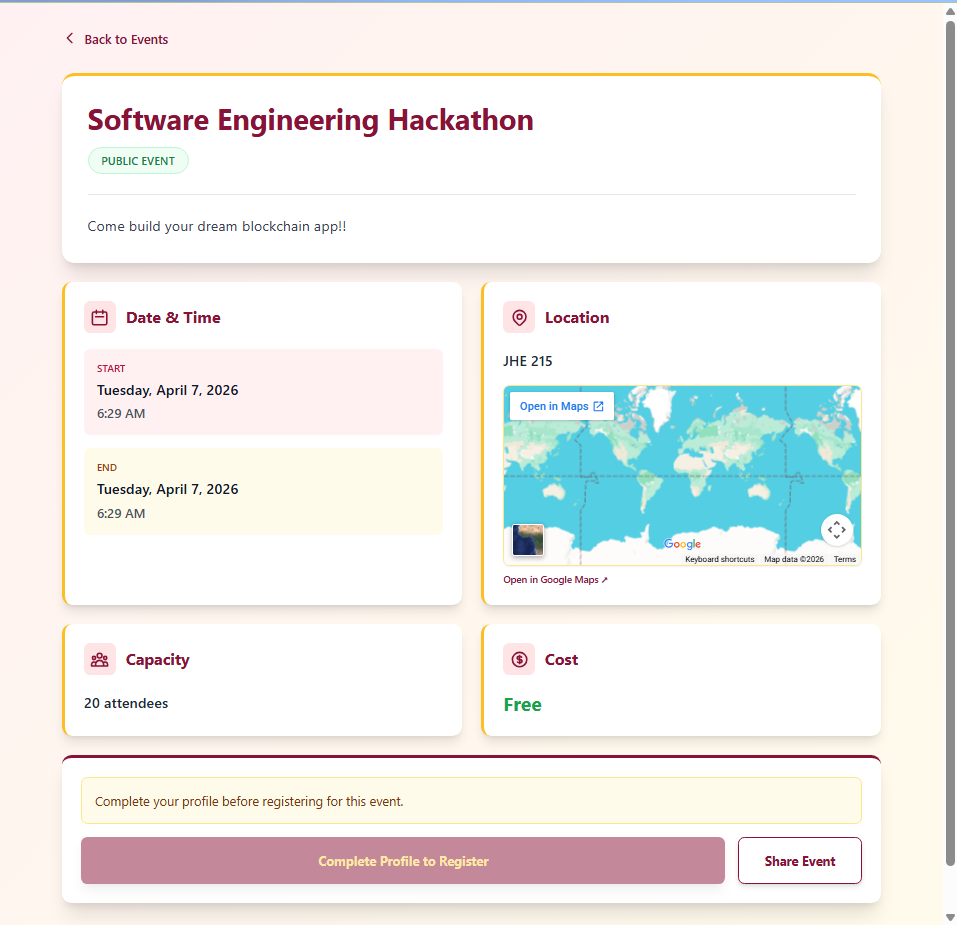
\includegraphics[width=\textwidth]{Images/Constraints2.1.png}
        \caption{Event registration blocked until profile is complete}
        \label{fig:constraints-profile-gate-events}
    \end{subfigure}
    \hfill
    \begin{subfigure}[t]{0.48\textwidth}
        \centering
        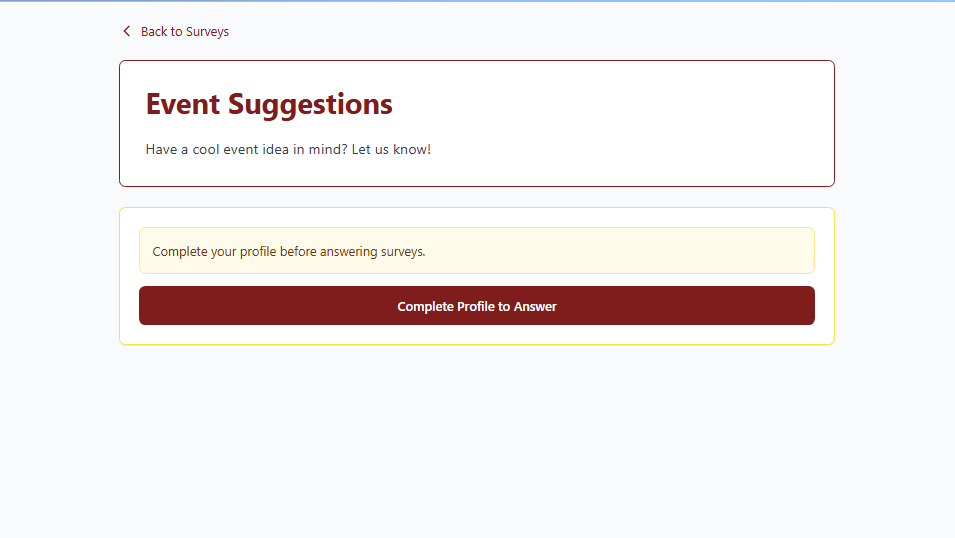
\includegraphics[width=\textwidth]{Images/Constraints2.2.png}
        \caption{Survey response blocked until profile is complete}
        \label{fig:constraints-profile-gate-surveys}
    \end{subfigure}
    \caption{Profile-completion constraint applied consistently to events and surveys}
    \label{fig:constraints-profile-gate}
\end{figure}

\subsection{Example 3 (Bad): Event and Form creation does not constrain invalid time ordering in the UI}
In the admin event creation flow, start and end times are required fields, but the interface does not enforce a clear constraint that end time must be later than start time before submission. This allows users to enter logically invalid time ranges and only discover issues later. The same issue is encountered when considering unlock dates in forms where a form can be set to be unlocked in the past without proper validation. This is a weak application of Constraints because the system does not prevent a common invalid input at the point of entry.

\begin{figure}[H]
    \centering
    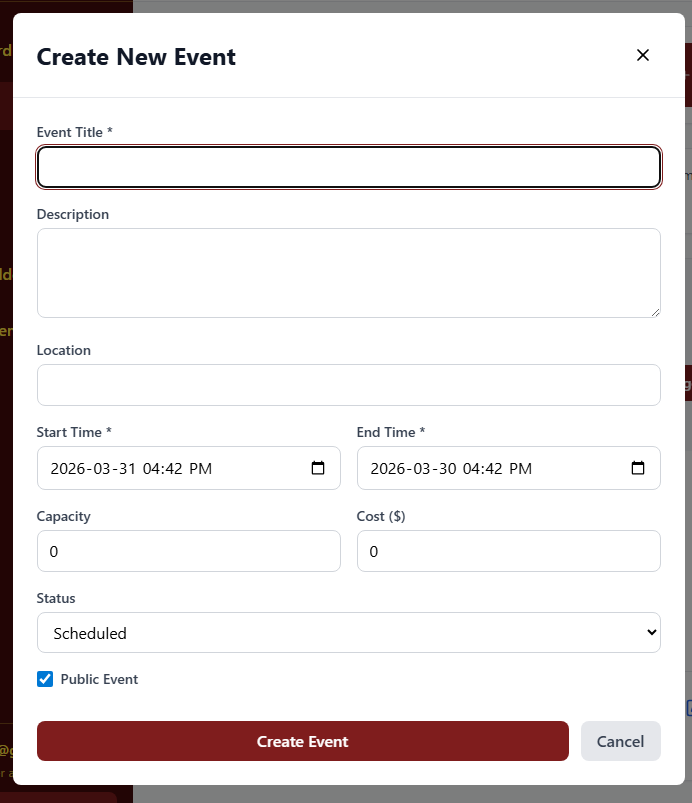
\includegraphics[width=0.9\textwidth]{Images/Constraints3.png}
    \caption{Admin event form allowing time inputs without explicit ordering constraint}
    \label{fig:constraints-event-time-order}
\end{figure}

\textbf{Recommendation:} Add front-end and back-end validation that enforces end time is greater than start time with immediate inline feedback near the fields. We could also put even stricter checks if neccesary to ensure that events and forms can't set to be open in the past. This would prevent invalid submissions earlier and reduce correction effort for admins.


\section{Consistency}
Consistency concerns whether similar elements behave and appear in similar ways across the platform.

\subsection{Example 1 (Good): Primary action styling is broadly consistent across key workflows}
Across both user and admin portals, major actions are typically presented as high-contrast, prominent buttons while lower-priority actions use secondary styling. This repeated visual hierarchy helps users quickly identify which action is primary when creating events, registering for events, or publishing content. This is a good application of consistency because users can transfer expectations between screens without relearning button priority each time and by looking at the buttons see the importance due to the different styling and look compared to the rest of the screens.

\begin{figure}[H]
    \centering
    \begin{subfigure}[t]{0.48\textwidth}
        \centering
        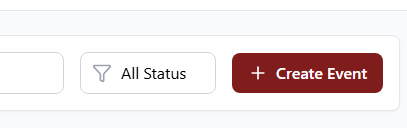
\includegraphics[width=\textwidth]{Images/Consistency1.1.png}
        \label{fig:consistency-primary-actions-a}
    \end{subfigure}
    \hfill
    \begin{subfigure}[t]{0.48\textwidth}
        \centering
        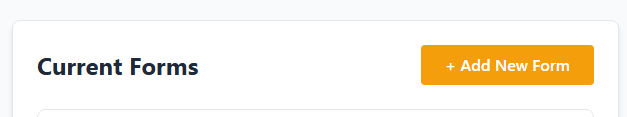
\includegraphics[width=\textwidth]{Images/Consistency1.2.png}
        \label{fig:consistency-primary-actions-b}
    \end{subfigure}

    \vspace{0.6em}

    \begin{subfigure}[t]{0.48\textwidth}
        \centering
        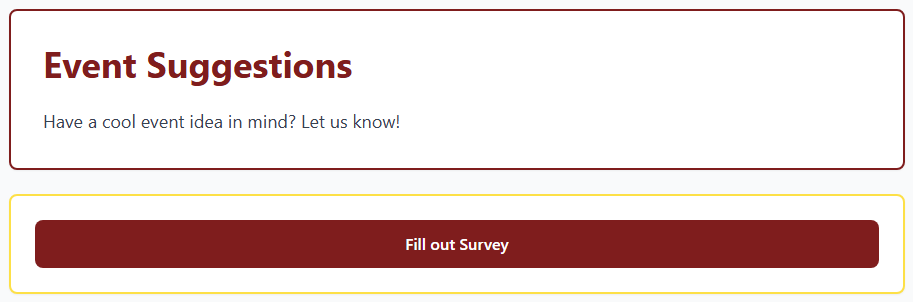
\includegraphics[width=\textwidth]{Images/Consistency1.3.png}
        \label{fig:consistency-primary-actions-c}
    \end{subfigure}
    \hfill
    \begin{subfigure}[t]{0.48\textwidth}
        \centering
        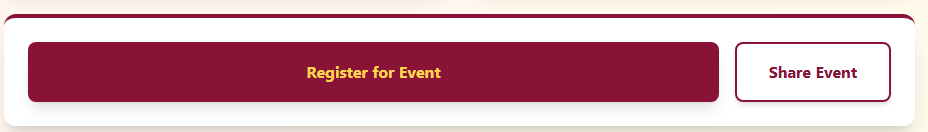
\includegraphics[width=\textwidth]{Images/Consistency1.4.png}
        \label{fig:consistency-primary-actions-d}
    \end{subfigure}
    \caption{Consistent button styling}
    \label{fig:consistency-primary-actions}
\end{figure}

\subsection{Example 2 (Bad): Confirmation dialogs are implemented inconsistently}
The platform uses multiple confirmation patterns for similar completion and confirmation actions: some pages use custom in-app confirmation modals while others still use the browser's native confirmation popup. For other situations we have specific submission pages to showcase workflow confirmations. Although both patterns prevent accidental actions, this inconsistency breaks interaction rhythm and can make the interface feel fragmented. This is a weak application of consistency because users do not receive the same confirmation experience for similar tasks.

\textbf{Recommendation:} Standardize  confirmations to use one shared in-app confirmation component (instead of mixing custom modals and browser popups) and keep button labels consistent. This would make the interaction pattern predictable across pages and reduce user hesitation. Another way that we could accomplish this is by either standardzing modal usage, alert usage or having ocnfirmation pages. Obviously some use cases don't require explicit pages but having a complete workflow requires some type of feedback or confirmation to ensure user's have an understadning that they have reached the end of the workflow.



\subsection{Example 3 (Bad): Status and error messaging patterns vary across pages}
The platform presents outcome messages in several different styles depending on page context, including toast notifications, inline banners, modal alerts, and native browser prompts. While each method can work individually, the mixed usage for similar success and failure outcomes creates an inconsistent communication pattern across workflows.

This is a weaker application of consistency because users cannot reliably predict where important feedback will appear or what visual style it will use after completing an action.

\begin{figure}[H]
    \centering
    \begin{subfigure}[t]{0.48\textwidth}
        \centering
        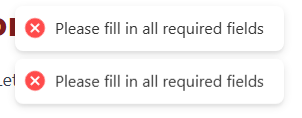
\includegraphics[width=\textwidth]{Images/Consistency3.1.png}
    \end{subfigure}
    \hfill
    \begin{subfigure}[t]{0.48\textwidth}
        \centering
        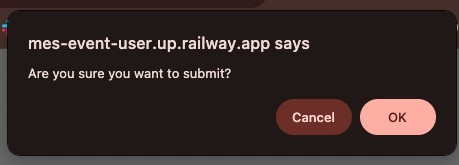
\includegraphics[width=\textwidth]{Images/Consistency3.2.jpg}
        \label{fig:feedback-survey-submission-right}
    \end{subfigure}
    \caption{Status and Error Messages}
\end{figure}
\textbf{Recommendation:} Define one platform-wide messaging standard (for example, inline banner for page-level results and toast for short non-blocking updates) and apply it consistently across user and admin portals. This will make outcomes easier to notice and interpret and show consistency and higher level of professionalism. Ideally this would be a custom component so that we could control the information and how we want to show and format the information.



\end{document}